% Options for packages loaded elsewhere
\PassOptionsToPackage{unicode}{hyperref}
\PassOptionsToPackage{hyphens}{url}
\PassOptionsToPackage{dvipsnames,svgnames,x11names}{xcolor}
%
\documentclass[
  letterpaper,
  DIV=11,
  numbers=noendperiod]{scrartcl}

\usepackage{amsmath,amssymb}
\usepackage{lmodern}
\usepackage{iftex}
\ifPDFTeX
  \usepackage[T1]{fontenc}
  \usepackage[utf8]{inputenc}
  \usepackage{textcomp} % provide euro and other symbols
\else % if luatex or xetex
  \usepackage{unicode-math}
  \defaultfontfeatures{Scale=MatchLowercase}
  \defaultfontfeatures[\rmfamily]{Ligatures=TeX,Scale=1}
\fi
% Use upquote if available, for straight quotes in verbatim environments
\IfFileExists{upquote.sty}{\usepackage{upquote}}{}
\IfFileExists{microtype.sty}{% use microtype if available
  \usepackage[]{microtype}
  \UseMicrotypeSet[protrusion]{basicmath} % disable protrusion for tt fonts
}{}
\makeatletter
\@ifundefined{KOMAClassName}{% if non-KOMA class
  \IfFileExists{parskip.sty}{%
    \usepackage{parskip}
  }{% else
    \setlength{\parindent}{0pt}
    \setlength{\parskip}{6pt plus 2pt minus 1pt}}
}{% if KOMA class
  \KOMAoptions{parskip=half}}
\makeatother
\usepackage{xcolor}
\setlength{\emergencystretch}{3em} % prevent overfull lines
\setcounter{secnumdepth}{-\maxdimen} % remove section numbering
% Make \paragraph and \subparagraph free-standing
\ifx\paragraph\undefined\else
  \let\oldparagraph\paragraph
  \renewcommand{\paragraph}[1]{\oldparagraph{#1}\mbox{}}
\fi
\ifx\subparagraph\undefined\else
  \let\oldsubparagraph\subparagraph
  \renewcommand{\subparagraph}[1]{\oldsubparagraph{#1}\mbox{}}
\fi


\providecommand{\tightlist}{%
  \setlength{\itemsep}{0pt}\setlength{\parskip}{0pt}}\usepackage{longtable,booktabs,array}
\usepackage{calc} % for calculating minipage widths
% Correct order of tables after \paragraph or \subparagraph
\usepackage{etoolbox}
\makeatletter
\patchcmd\longtable{\par}{\if@noskipsec\mbox{}\fi\par}{}{}
\makeatother
% Allow footnotes in longtable head/foot
\IfFileExists{footnotehyper.sty}{\usepackage{footnotehyper}}{\usepackage{footnote}}
\makesavenoteenv{longtable}
\usepackage{graphicx}
\makeatletter
\def\maxwidth{\ifdim\Gin@nat@width>\linewidth\linewidth\else\Gin@nat@width\fi}
\def\maxheight{\ifdim\Gin@nat@height>\textheight\textheight\else\Gin@nat@height\fi}
\makeatother
% Scale images if necessary, so that they will not overflow the page
% margins by default, and it is still possible to overwrite the defaults
% using explicit options in \includegraphics[width, height, ...]{}
\setkeys{Gin}{width=\maxwidth,height=\maxheight,keepaspectratio}
% Set default figure placement to htbp
\makeatletter
\def\fps@figure{htbp}
\makeatother

\KOMAoption{captions}{tableheading}
\makeatletter
\@ifpackageloaded{tcolorbox}{}{\usepackage[many]{tcolorbox}}
\@ifpackageloaded{fontawesome5}{}{\usepackage{fontawesome5}}
\definecolor{quarto-callout-color}{HTML}{909090}
\definecolor{quarto-callout-note-color}{HTML}{0758E5}
\definecolor{quarto-callout-important-color}{HTML}{CC1914}
\definecolor{quarto-callout-warning-color}{HTML}{EB9113}
\definecolor{quarto-callout-tip-color}{HTML}{00A047}
\definecolor{quarto-callout-caution-color}{HTML}{FC5300}
\definecolor{quarto-callout-color-frame}{HTML}{acacac}
\definecolor{quarto-callout-note-color-frame}{HTML}{4582ec}
\definecolor{quarto-callout-important-color-frame}{HTML}{d9534f}
\definecolor{quarto-callout-warning-color-frame}{HTML}{f0ad4e}
\definecolor{quarto-callout-tip-color-frame}{HTML}{02b875}
\definecolor{quarto-callout-caution-color-frame}{HTML}{fd7e14}
\makeatother
\makeatletter
\makeatother
\makeatletter
\makeatother
\makeatletter
\@ifpackageloaded{caption}{}{\usepackage{caption}}
\AtBeginDocument{%
\ifdefined\contentsname
  \renewcommand*\contentsname{Table of contents}
\else
  \newcommand\contentsname{Table of contents}
\fi
\ifdefined\listfigurename
  \renewcommand*\listfigurename{List of Figures}
\else
  \newcommand\listfigurename{List of Figures}
\fi
\ifdefined\listtablename
  \renewcommand*\listtablename{List of Tables}
\else
  \newcommand\listtablename{List of Tables}
\fi
\ifdefined\figurename
  \renewcommand*\figurename{Figure}
\else
  \newcommand\figurename{Figure}
\fi
\ifdefined\tablename
  \renewcommand*\tablename{Table}
\else
  \newcommand\tablename{Table}
\fi
}
\@ifpackageloaded{float}{}{\usepackage{float}}
\floatstyle{ruled}
\@ifundefined{c@chapter}{\newfloat{codelisting}{h}{lop}}{\newfloat{codelisting}{h}{lop}[chapter]}
\floatname{codelisting}{Listing}
\newcommand*\listoflistings{\listof{codelisting}{List of Listings}}
\makeatother
\makeatletter
\@ifpackageloaded{caption}{}{\usepackage{caption}}
\@ifpackageloaded{subcaption}{}{\usepackage{subcaption}}
\makeatother
\makeatletter
\@ifpackageloaded{tcolorbox}{}{\usepackage[many]{tcolorbox}}
\makeatother
\makeatletter
\@ifundefined{shadecolor}{\definecolor{shadecolor}{rgb}{.97, .97, .97}}
\makeatother
\makeatletter
\makeatother
\ifLuaTeX
  \usepackage{selnolig}  % disable illegal ligatures
\fi
\IfFileExists{bookmark.sty}{\usepackage{bookmark}}{\usepackage{hyperref}}
\IfFileExists{xurl.sty}{\usepackage{xurl}}{} % add URL line breaks if available
\urlstyle{same} % disable monospaced font for URLs
\hypersetup{
  pdftitle={Álgebra Linear Computacional},
  pdfauthor={Heitor S. Ramos   ramosh@dcc.ufmg.br},
  colorlinks=true,
  linkcolor={blue},
  filecolor={Maroon},
  citecolor={Blue},
  urlcolor={Blue},
  pdfcreator={LaTeX via pandoc}}

\title{Álgebra Linear Computacional}
\usepackage{etoolbox}
\makeatletter
\providecommand{\subtitle}[1]{% add subtitle to \maketitle
  \apptocmd{\@title}{\par {\large #1 \par}}{}{}
}
\makeatother
\subtitle{Aula 07: Normas de Vetores e Matrizes - Parte II}
\author{Heitor S. Ramos ramosh@dcc.ufmg.br}
\date{}

\begin{document}
\maketitle
\ifdefined\Shaded\renewenvironment{Shaded}{\begin{tcolorbox}[boxrule=0pt, borderline west={3pt}{0pt}{shadecolor}, enhanced, breakable, sharp corners, frame hidden, interior hidden]}{\end{tcolorbox}}\fi

\hypertarget{cruxe9ditos}{%
\subsection{Créditos}\label{cruxe9ditos}}

\begin{tcolorbox}[enhanced jigsaw, title=\textcolor{quarto-callout-important-color}{\faExclamation}\hspace{0.5em}{Important}, arc=.35mm, left=2mm, leftrule=.75mm, toprule=.15mm, colbacktitle=quarto-callout-important-color!10!white, bottomrule=.15mm, rightrule=.15mm, titlerule=0mm, breakable, colframe=quarto-callout-important-color-frame, opacitybacktitle=0.6, toptitle=1mm, opacityback=0, colback=white, bottomtitle=1mm, coltitle=black]
Os slides desse curso são fortemente baseados no curso do Fabrício Murai
e do Erickson Nascimento
\end{tcolorbox}

\hypertarget{objetivos}{%
\subsection{Objetivos}\label{objetivos}}

\begin{enumerate}
\def\labelenumi{\arabic{enumi}.}
\tightlist
\item
  Conhecer a definição de distância estatística
\item
  Conhecer relação entre normais vetoriais e normas matriciais induzidas
\item
  Saber calcular normas matriciais 1, 2, de Frobenius, infinito
\item
  Conhecer propriedades de normas matriciais
\item
  Saber interpretar a norma espectral (norma-2 matricial)
\end{enumerate}

\hypertarget{referuxeancias-adicionais}{%
\subsection{Referências adicionais}\label{referuxeancias-adicionais}}

\begin{itemize}
\tightlist
\item
  Wikipedia

  \begin{itemize}
  \tightlist
  \item
    \href{https://en.wikipedia.org/wiki/Norm_(mathematics)}{Normas
    matriciais}
  \item
    \href{https://en.wikipedia.org/wiki/Norm_(mathematics)}{Normas
    vetoriais}
  \end{itemize}
\item
  Youtube

  \begin{itemize}
  \tightlist
  \item
    \href{https://youtu.be/UtNPmGw60jg}{Chad Higdon-Topaz}
  \end{itemize}
\end{itemize}

\hypertarget{distuxe2ncia-estatuxedstica}{%
\subsection{Distância estatística}\label{distuxe2ncia-estatuxedstica}}

\begin{itemize}
\tightlist
\item
  Precisamos de uma distância diferente da euclidiana para detectar
  anomalias em dados
\item
  Vamos começar vendo matrizes de dados estatísticos: matrizes com n
  items e k colunas ou variáveis
\end{itemize}

\hypertarget{exemplo-1}{%
\subsection{Exemplo 1}\label{exemplo-1}}

\begin{itemize}
\tightlist
\item
  Relação entre força de preensão (do aperto de mão) e força do braço
  para 147 pessoas que trabalham em empregos fisicamente extenuantes
\end{itemize}

\begin{figure}

{\centering 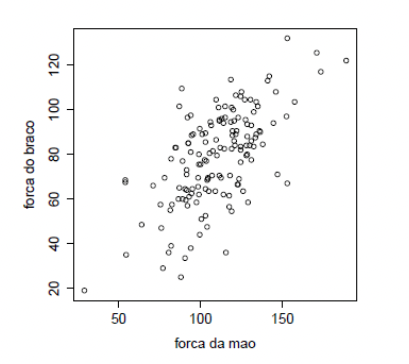
\includegraphics{figs/Aula07/ex1.png}

}

\end{figure}

\hypertarget{matrizes-de-dados}{%
\subsection{Matrizes de dados}\label{matrizes-de-dados}}

Um vetor para cada indivíduo \(y = (y_1,y_2,\ldots,y_n)\)

As 9 variáveis são escores obtidos em 9 testes de habilidade cognitiva:

\begin{itemize}
\tightlist
\item
  3 medindo habilidade verbal: Word Meaning, Sentence Completion, and
  Odd words
\item
  3 medindo habilidade quantitativa: Mixed Arithmetic, Remainders, and
  Missing numbers
\item
  3 medindo habilidade espacial: Gloves, Boots, and Hatchets
\end{itemize}

\hypertarget{matrizes-de-dados-1}{%
\subsection{Matrizes de dados}\label{matrizes-de-dados-1}}

\begin{figure}

{\centering 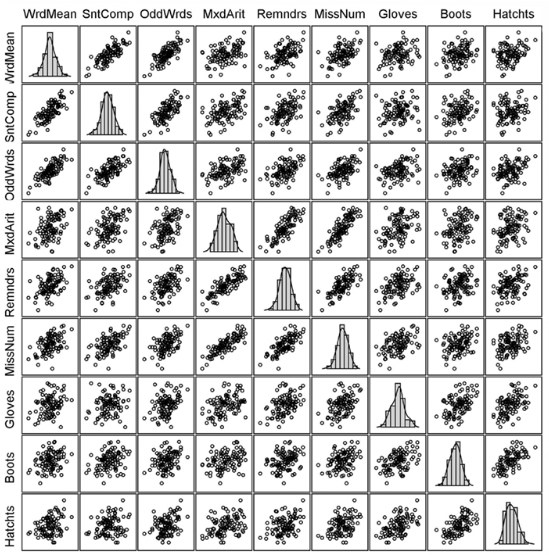
\includegraphics{figs/Aula07/ex2.png}

}

\end{figure}

\hypertarget{matriz-de-correlauxe7uxe3o}{%
\subsection{Matriz de correlação}\label{matriz-de-correlauxe7uxe3o}}

\begin{figure}

{\centering 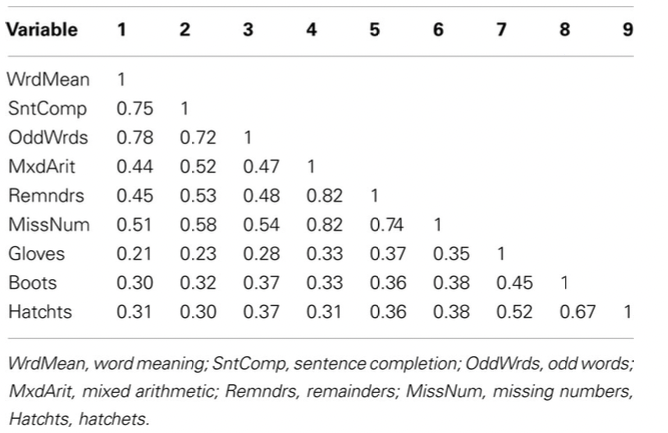
\includegraphics{figs/Aula07/Mcorr.png}

}

\end{figure}

\begin{itemize}
\tightlist
\item
  Matriz simétrica e definida positiva
\item
  Elemento \((i,j)\) mede o grau de associação linear entre um par de
  variáveis (diagonal 1, por quê?)
\end{itemize}

\hypertarget{desvio-padruxe3o}{%
\subsection{Desvio padrão}\label{desvio-padruxe3o}}

\begin{itemize}
\tightlist
\item
  Desvio padrão (\(\sigma\)) é o tamanho médio do desvio de um dado para
  a média
\end{itemize}

\begin{figure}

{\centering 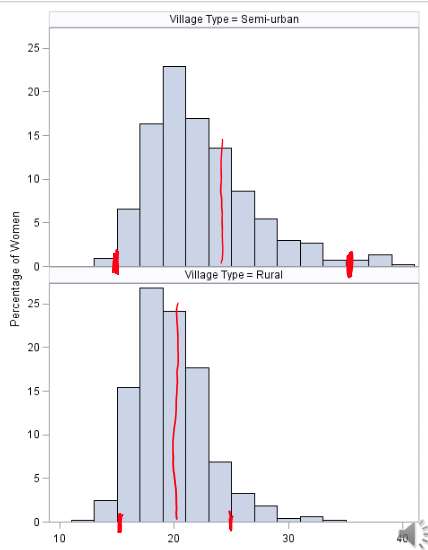
\includegraphics{figs/Aula07/desviopadrao.png}

}

\end{figure}

\hypertarget{pressuxe3o-sistuxf3lica}{%
\subsection{Pressão sistólica}\label{pressuxe3o-sistuxf3lica}}

\begin{itemize}
\tightlist
\item
  A pressão sistólica mede a força do sangue nas artérias à medida que o
  coração contrai para impulsionar o sangue
\item
  Se alta, ela pode levar à doença do coração, anginas e doenças
  vasculares nas pernas
\item
  Pressão sistólica saudável: entre 120 e 140 mmHg
\item
  Pressão sisólica \textgreater{} 140 mmHg: não saudável
\item
  Pressão diastólica deve ficar em torno de 80
\item
  Acima de 100 não é saudável
\end{itemize}

\hypertarget{pressuxe3o-de-250-indivuxedduos}{%
\subsection{Pressão de 250
indivíduos}\label{pressuxe3o-de-250-indivuxedduos}}

\begin{figure}

{\centering 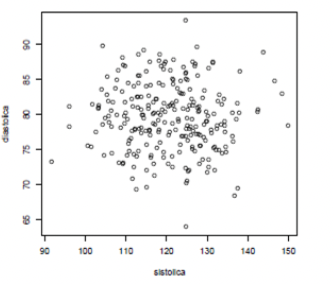
\includegraphics[width=0.55\textwidth,height=\textheight]{figs/Aula07/pressao.png}

}

\caption{Amostra de \((y_{i1}, y_{i2})\), com \(i = 1,2,\ldots, 250\)}

\end{figure}

\hypertarget{muxe9dias-para-referuxeancia}{%
\subsection{Médias para referência}\label{muxe9dias-para-referuxeancia}}

\begin{itemize}
\tightlist
\item
  250 instâncias do vetor aleatório: \(Y = (Y_1, Y_2)\)
\item
  Vetor com os valores esperados de cada variável:
\end{itemize}

\[\mathbb E(Y) = \mathbb E(Y_1,Y_2) = (\mathbb E(Y_1), \mathbb E(Y_2)) = (\mu_1, \mu_2) = \mu\]

\begin{figure}

{\centering 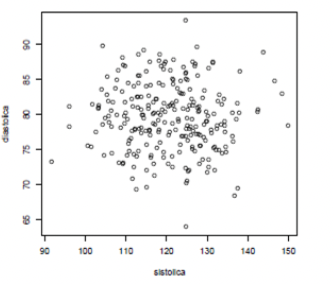
\includegraphics[width=0.55\textwidth,height=\textheight]{figs/Aula07/pressao.png}

}

\end{figure}

\hypertarget{quem-estuxe1-distante-do-esperado}{%
\subsection{Quem está distante do
esperado?}\label{quem-estuxe1-distante-do-esperado}}

\begin{itemize}
\tightlist
\item
  Centro \(\mu = (\mu_1, \mu_2)\) é o perfil esperado ou típico
\item
  Quem está longe do perfil típico? Quem é anômalo?
\item
  Medida baseada na distância euclidiana
  \(d(y_1,y_2) = \sqrt{(y_1-120)^2+ (y_2-80)^2}\)
\item
  é razoável?
\end{itemize}

\begin{figure}

{\centering 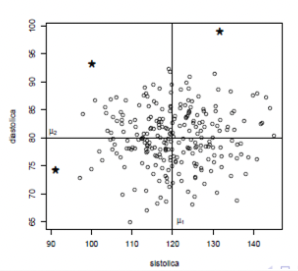
\includegraphics[width=0.55\textwidth,height=\textheight]{figs/Aula07/distancia_pressao.png}

}

\end{figure}

\hypertarget{exagerando-um-pouco}{%
\subsection{Exagerando um pouco}\label{exagerando-um-pouco}}

\begin{itemize}
\tightlist
\item
  E se o segundo atributo for assim? Fazendo o
  \(\text{aspect/ratio} = 1\).
\item
  Centro \(\mu = (\mu_1, \mu_2)\) continua o mesmo
\item
  Mas quem está distante do centro agora? Quem é anômalo?
\end{itemize}

\begin{figure}

{\centering 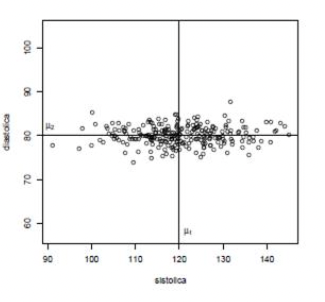
\includegraphics[width=0.55\textwidth,height=\textheight]{figs/Aula07/pressao2.png}

}

\end{figure}

\hypertarget{distantes-suxe3o-uxf3bvios-nuxe3o}{%
\subsection{Distantes são óbvios,
não?}\label{distantes-suxe3o-uxf3bvios-nuxe3o}}

\begin{itemize}
\tightlist
\item
  Mas qual é a medida de distância que estamos usando sem ao mesmo
  perceber?
\item
  Não é a distância euclidiana!
\end{itemize}

\begin{figure}

{\centering 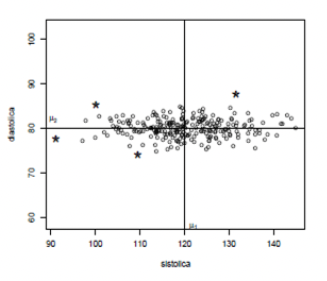
\includegraphics[width=0.55\textwidth,height=\textheight]{figs/Aula07/distancia_pressao2.png}

}

\end{figure}

\hypertarget{pontos-uxe0-igual-distuxe2ncia}{%
\subsection{Pontos à igual
distância}\label{pontos-uxe0-igual-distuxe2ncia}}

\begin{itemize}
\tightlist
\item
  Todos os pontos do círculo estão à igual distância do centro da nuvem
  de pontos
\item
  Queremos os dois pontos em vermelho à igual distância
  \textbf{ESTATÍSTICA} do centro que os pontos em azul?
\item
  \textbf{NÃO!} Pontos vermelhos estão \textbf{ESTATISTICAMENTE} muito
  mais distantes do centro \((\mu_1, \mu_2)\) do que os pontos azuis
\end{itemize}

\begin{figure}

{\centering 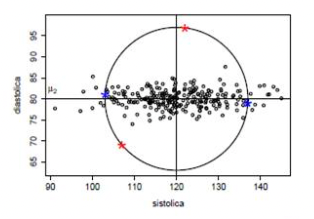
\includegraphics[width=0.55\textwidth,height=\textheight]{figs/Aula07/distancia_centro.png}

}

\end{figure}

\hypertarget{pontos-vermelhos-mais-distantes}{%
\subsection{Pontos vermelhos mais
distantes}\label{pontos-vermelhos-mais-distantes}}

\begin{itemize}
\tightlist
\item
  Como fazer os pontos vermelhos mais distantes que os pontos azuis?
\item
  Andar poucas unidades na direção norte-sul te leva pra fora da nuvem
  dos pontos (vira anomalia)
\item
  Precisa andar \textbf{MAIS} unidades na direção leste-oeste para sair
  da nuvem de pontos
\end{itemize}

\begin{figure}

{\centering 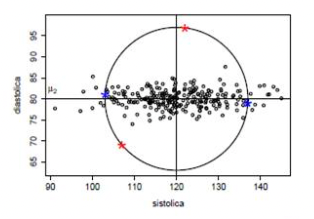
\includegraphics[width=0.55\textwidth,height=\textheight]{figs/Aula07/distancia_centro.png}

}

\end{figure}

\hypertarget{pontos-vermelhos-mais-distantes-1}{%
\subsection{Pontos vermelhos mais
distantes}\label{pontos-vermelhos-mais-distantes-1}}

\begin{itemize}
\tightlist
\item
  Então \(N\) unidades euclidianas na direção leste-oeste valem o
  \textbf{MESMO} que \(N/k\) na direção norte-sul (onde \(k>1\))
\item
  Como achar esse \(k\)?
\item
  Como equalizar as distâncias?
\item
  \textbf{Resposta:} Medindo distâncias em unidades de \textbf{DESVIOS
  PADRÕES}
\end{itemize}

\begin{figure}

{\centering 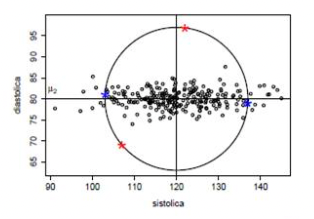
\includegraphics[width=0.55\textwidth,height=\textheight]{figs/Aula07/distancia_centro.png}

}

\end{figure}

\hypertarget{medida-de-dispersuxe3o}{%
\subsection{Medida de dispersão}\label{medida-de-dispersuxe3o}}

\begin{itemize}
\tightlist
\item
  Desvio padrão DP: um para cada eixo, um para cada atributo
\item
  DP mede quanto, em média, um atributo aleatório desvia-se do seue
  valor esperado
\item
  Por exemplo, \(DP=10\) significa:

  \begin{itemize}
  \tightlist
  \item
    Em geral, observações desviam-se de 10 unidades em torno do seu
    valor esperado
  \item
    Às vezes mais de 10 unidades; às vezes menos de 10 unidades
  \item
    Em média, um afastamento de 10 unidades
  \end{itemize}
\end{itemize}

\hypertarget{qual-o-desvio-padruxe3o-de-cada-variuxe1vel}{%
\subsection{Qual o desvio padrão de cada
variável?}\label{qual-o-desvio-padruxe3o-de-cada-variuxe1vel}}

\begin{itemize}
\tightlist
\item
  Centro \(\mathbb E(Y) = \mu = (\mu_1, \mu_2) = (120,80)\)
\item
  \(DP_1 = \sigma_1 = ??\)
\item
  \(DP_2 = \sigma_2 = ??\)
\end{itemize}

\begin{figure}

{\centering 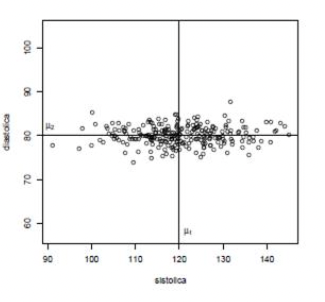
\includegraphics[width=0.55\textwidth,height=\textheight]{figs/Aula07/pressao2.png}

}

\end{figure}

\hypertarget{qual-o-desvio-padruxe3o-de-cada-variuxe1vel-1}{%
\subsection{Qual o desvio padrão de cada
variável?}\label{qual-o-desvio-padruxe3o-de-cada-variuxe1vel-1}}

\begin{itemize}
\tightlist
\item
  Centro \(\mathbb E(Y) = \mu = (\mu_1, \mu_2) = (120,80)\)
\item
  \(DP_1 = \sigma_1 = 10\)
\item
  \(DP_2 = \sigma_2 = 2\)
\end{itemize}

\begin{figure}

{\centering 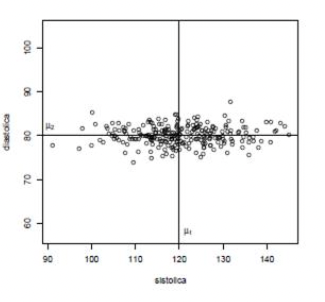
\includegraphics[width=0.55\textwidth,height=\textheight]{figs/Aula07/pressao2.png}

}

\end{figure}

\hypertarget{distuxe2ncia-medida-em-dp}{%
\subsection{Distância medida em DP}\label{distuxe2ncia-medida-em-dp}}

\begin{itemize}
\tightlist
\item
  \((\mu_1,\mu_2) = (120,80)\) e \((\sigma_1, \sigma_2) = (10,2)\)
\item
  AZUL: afastou-se do centro apenas ao longo do eixo 1 e afastou-se
  \(15\) unidades, ou \(1.5\sigma_1\)
\item
  VERMELHO: afastou-se do centro apenas ao longo do eixo 2 e afastou-se
  \(15\) unidades ou \(7.5\sigma_2\)
\item
  o ponto VERMELHO está muito mais distante do centro em termos de DPs
\item
  Mas como fazer com pontos que afastam-se do centro não somente ao
  longo de um dos eixos?
\end{itemize}

\begin{figure}

{\centering 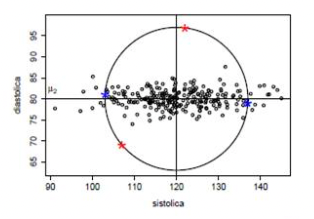
\includegraphics[width=0.55\textwidth,height=\textheight]{figs/Aula07/distancia_centro.png}

}

\end{figure}

\hypertarget{distuxe2ncia-medida-em-dp-1}{%
\subsection{Distância medida em DP}\label{distuxe2ncia-medida-em-dp-1}}

\begin{itemize}
\tightlist
\item
  \((\mu_1,\mu_2) = (120,80)\) e \((\sigma_1, \sigma_2) = (10,2)\)
\item
  Andar \(n\sigma_1\) ao longo do eixo 1 é EQUIVALENTE a andar
  \(n\sigma_2\) no eixo 2
\item
  Por exemplo, 20 unidades ao longo do eixo 1 (ou \(2\sigma_1\)) é
  ESTATISTICAMENTE EQUIVALENTE a 4 unidades ao (ou \(2\sigma_2\)) longo
  do eixo 2
\end{itemize}

\begin{figure}

{\centering 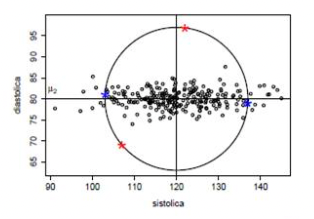
\includegraphics[width=0.55\textwidth,height=\textheight]{figs/Aula07/distancia_centro.png}

}

\end{figure}

\hypertarget{distuxe2ncia-medida-em-dp-2}{%
\subsection{Distância medida em DP}\label{distuxe2ncia-medida-em-dp-2}}

\begin{itemize}
\tightlist
\item
  Vamos medir o desvio em cada eixo EM UNIDADES DE DESVIO PADRÃO e
  calcular a distância com esses desvios padronizados
\item
  DESVIO PADRONIZADO ao longo do eixo 1
  \[z_1 = \frac{y_1 - \mu_1}{\sigma_1}= \frac{y_1-120}{10}\]
\item
  DESVIO PADRONIZADO ao longo do eixo 2
  \[z_2 = \frac{y_2 - \mu_2}{\sigma_2}= \frac{y_2-80}{2}\]
\item
  Distância:
\end{itemize}

\begin{align} 
d(y_1,y_2) &= \sqrt{z_1^2 + z_2^2} \\
&= \sqrt{\left(\frac{y_1-120}{10}\right)^2 + \left(\frac{y_2-80}{2}\right)^2} \\
&= \sqrt{\left(\frac{y_1-\mu_1}{\sigma_1}\right)^2 + \left(\frac{y_2-\mu_2}{\sigma_2}\right)^2} \\
\end{align}

\hypertarget{pontos-a-igual-distuxe2ncia}{%
\subsection{Pontos a igual
distância}\label{pontos-a-igual-distuxe2ncia}}

\begin{itemize}
\tightlist
\item
  NESSA NOVA MÉTRICA, quais os pontos \((y_1, y_2)\) que estão a uma
  MESMA distância do centro \((\mu_1, \mu_2)\)?
\item
  Tome uma distância fixa (por exemplo, 1)
\item
  Eles formam uma ELIPSE centrada em \((\mu_1, \mu_2)\) e com eixos
  paralelos aos eixos coordenados
\end{itemize}

\[ d(y, \mu)  = \sqrt{\left(\frac{y_1-120}{10}\right)^2 + \left(\frac{y_2-80}{2}\right)^2} =1 \]

\begin{figure}

{\centering 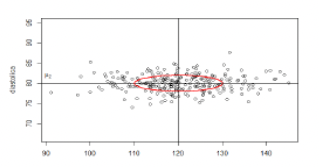
\includegraphics[width=0.55\textwidth,height=\textheight]{figs/Aula07/elipse.png}

}

\end{figure}

\hypertarget{tamanho-dos-eixos}{%
\subsection{Tamanho dos eixos}\label{tamanho-dos-eixos}}

\begin{itemize}
\tightlist
\item
  Distância \(c>0\) do centro: pontos satisfazem a equação
\end{itemize}

\[ d(y, \mu)  = \sqrt{\left(\frac{y_1-120}{10}\right)^2 + \left(\frac{y_2-80}{2}\right)^2} =c \]

\begin{itemize}
\tightlist
\item
  Os eixos têm comprimentos iguais a \(c\sigma_1\) e \(c\sigma_2\). O
  eixo maior da elipse: variável com maior DP
\item
  Quantas vezes o maior eixo é maior que o eixo menor?
\item
  Se \(\sigma_1\) é o maior DP,
\end{itemize}

\[\frac{\text{eixo maior}}{\text{eixo menor}} = \frac{c\sigma_1}{c\sigma2} = \frac{\sigma1}{\sigma_2}\]

\begin{itemize}
\tightlist
\item
  Não depende da distância \(c\). Ao variarmos \(c\) teremos elipses
  concêntricas
\end{itemize}

\hypertarget{variando-a-distuxe2ncia}{%
\subsection{Variando a distância}\label{variando-a-distuxe2ncia}}

\begin{figure}

{\centering 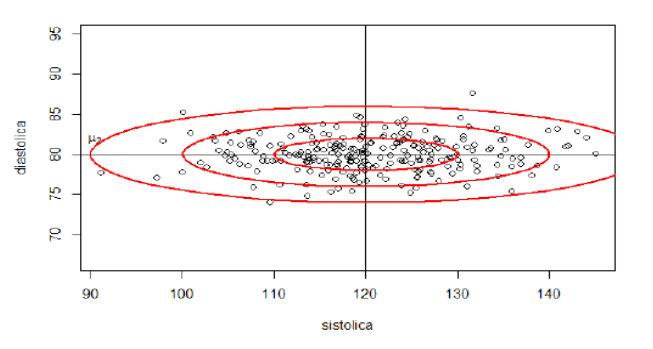
\includegraphics[width=0.8\textwidth,height=\textheight]{figs/Aula07/distancias.png}

}

\caption{Pontos \((y_1, y_2)\) que estão a uma distância \(c\) igual a
1, 2, 3 do centro \((\mu_1, \mu_2)\)}

\end{figure}

\hypertarget{jogando-fora-a-raiz-quadrada}{%
\subsection{Jogando fora a raiz
quadrada}\label{jogando-fora-a-raiz-quadrada}}

\begin{itemize}
\tightlist
\item
  Preferimos trabalhar com a distância AO QUADRADO
\item
  Se podemos complicar, por que simplificar?
\end{itemize}

\begin{align}
d^2(y,\mu) &= \left(\frac{y_1-\mu_1}{\sigma_1}\right)^2 + \left(\frac{y_2-\mu_2}{\sigma_2}\right)^2 \\
&= \begin{bmatrix}y_1 - \mu_1& y_2- \mu_2\end{bmatrix} \begin{bmatrix}1/\sigma_1 & 0 \\ 0 & 1/\sigma_2\end{bmatrix}\begin{bmatrix}y_1 - \mu_1 \\ y_2 - \mu_2\end{bmatrix}\\
&= \begin{bmatrix}y_1 - \mu_1& y_2- \mu_2\end{bmatrix} \begin{bmatrix}\sigma_1 & 0 \\ 0 & \sigma_2\end{bmatrix}^{-1}\begin{bmatrix}y_1 - \mu_1 \\ y_2 - \mu_2\end{bmatrix}\\
&= (y-\mu)^\top \Sigma^{-1}(y-\mu)
\end{align}

\hypertarget{elipses-e-distuxe2ncias}{%
\subsection{Elipses e distâncias}\label{elipses-e-distuxe2ncias}}

-Vimos que \begin{align}
d^2(y,\mu) &= \left(\frac{y_1-\mu_1}{\sigma_1}\right)^2 + \left(\frac{y_2-\mu_2}{\sigma_2}\right)^2 \\
&= (y-\mu)^\top \Sigma^{-1}(y-\mu)
\end{align} onde

\[ \Sigma = \begin{bmatrix} \sigma_1^2 & 0 \\ 0 & \sigma_2^2\end{bmatrix}\]

é a equação de uma elipse centrada em \(\mu = (\mu_1, \mu_2)\)

\begin{itemize}
\tightlist
\item
  Quando a matriz \(\Sigma\) é DIAGONAL com elementos positivos (com as
  variâncias \(\sigma_i\)'s), então a elipse tem eixos paralelos aos
  eixos e o tamanho de cada eixo é proporcional ao \(\sigma_i\) da
  variável associada
\end{itemize}

\hypertarget{caso-mais-realista}{%
\subsection{Caso mais realista}\label{caso-mais-realista}}

\begin{itemize}
\tightlist
\item
  Variáveis são associadas, não são independentes
\item
  Dizemos que são correlacionadas: redundância da informação
\item
  O valor de uma variável dá informação sobre o valor da outra variável
\item
  Pode-se predizer (com algum erro) uma variável em função da outra
\end{itemize}

\begin{figure}

{\centering 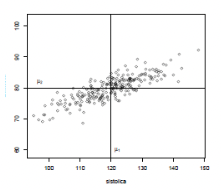
\includegraphics[width=0.55\textwidth,height=\textheight]{figs/Aula07/caso_mais_realista.png}

}

\end{figure}

\hypertarget{distuxe2ncia-eluxedptica-e-nuxe3o-circular}{%
\subsection{Distância elíptica e não
circular}\label{distuxe2ncia-eluxedptica-e-nuxe3o-circular}}

\begin{itemize}
\tightlist
\item
  Pelo mesmo raciocínio intuitivo que fizemos anteriormente, a ELIPSE
  abaixo tende a estar a igual distância do perfil esperado
  \(\mathbb E(Y) = \mu = (\mu_1,\mu_2)\)
\item
  Pontos estatisticamente equidistantes de \(\mu\) NÃO estão mais numa
  elipse paralela aos eixos
\item
  A elipse está inclinada seguindo a associação entre as variáveis
\end{itemize}

\begin{figure}

{\centering 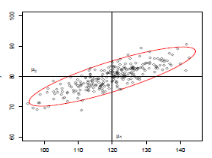
\includegraphics[width=0.55\textwidth,height=\textheight]{figs/Aula07/caso_mais_realista2.png}

}

\end{figure}

\hypertarget{forma-quadruxe1tica}{%
\subsection{Forma quadrática}\label{forma-quadruxe1tica}}

\begin{itemize}
\tightlist
\item
  Medida de distância é uma FORMA QUADRÁTICA
\end{itemize}

\[ d^2(y,\mu) = (y-\mu)^\top \Sigma^{-1}(y-\mu)\]

\begin{itemize}
\tightlist
\item
  É a memsa expressão matricial de distância que usamos antes
  MAS\ldots{}
\item
  \ldots{} a matriz \sigma não é mais DIAGONAL
\end{itemize}

\begin{figure}

{\centering 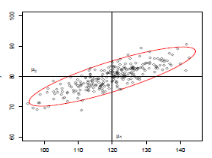
\includegraphics[width=0.55\textwidth,height=\textheight]{figs/Aula07/caso_mais_realista2.png}

}

\end{figure}

\hypertarget{quem-uxe9-sigma}{%
\subsection{\texorpdfstring{Quem é
\(\Sigma\)?}{Quem é \textbackslash Sigma?}}\label{quem-uxe9-sigma}}

\begin{itemize}
\tightlist
\item
  Medida de distância é uma FORMA QUADRÁTICA
\end{itemize}

\[ d^2(y,\mu) = (y-\mu)^\top \Sigma^{-1}(y-\mu)\]

\begin{itemize}
\tightlist
\item
  Matriz \(\Sigma\) é uma matriz \(2\times 2\) simétrica chamada de
  matriz de covariância
\end{itemize}

\[ \Sigma = \begin{bmatrix}\sigma_1^2 & \rho\sigma_1\sigma_2\\ \rho\sigma_1\sigma_2 & \sigma_2^2\end{bmatrix}\]

onde \(\rho = \text{Corr}(Y_1, Y_2)\) é o índice de correlação de
Pearson entre \(Y_1\) e \(Y_2\)

\begin{itemize}
\tightlist
\item
  Temos sempre \(-1 \le \rho \le 1\)
\item
  Os elementos fora da diagonal, \(\rho\sigma_1\sigma_2\), são chamados
  de covariância entre \(Y_1\) e \(Y_2\)
\item
  Costumamos escrever
  \(\text{Cov}(Y_1,Y_2) = \rho\sigma_1\sigma_2 = \sigma_{12}\)
\end{itemize}

\hypertarget{relauxe7uxe3o-entre-sigma-e-a-elipse}{%
\subsection{\texorpdfstring{Relação entre \(\Sigma\) e a
elipse}{Relação entre \textbackslash Sigma e a elipse}}\label{relauxe7uxe3o-entre-sigma-e-a-elipse}}

\begin{itemize}
\tightlist
\item
  distância é
\end{itemize}

\[ d^2(y,\mu) = (y-\mu)^\top \Sigma^{-1}(y-\mu)\]

onde \(\Sigma\) é uma matriz \(2\times 2\) simétrica dada por

\[ \Sigma = \begin{bmatrix}\sigma_1^2 & \rho\sigma_1\sigma_2\\ \rho\sigma_1\sigma_2 & \sigma_2^2\end{bmatrix}\]

\begin{itemize}
\tightlist
\item
  Pontos equidistantes de \(\mu = (\mu_1, \mu_2)\) estão numa elipse
\item
  Eixos da elipse: na direção dos AUTOVETORES da matriz \(\Sigma^{-1}\)
\item
  O tamanho de cada eixo é proporcional à raiz do AUTOVALOR
  correspondente
\end{itemize}

\begin{figure}

{\centering 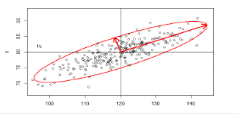
\includegraphics[width=0.55\textwidth,height=\textheight]{figs/Aula07/eigen_cov.png}

}

\end{figure}

\hypertarget{autovetor-e-autovalor-de-sigma-1}{%
\subsection{\texorpdfstring{Autovetor e autovalor de
\(\Sigma^{-1}\)}{Autovetor e autovalor de \textbackslash Sigma\^{}\{-1\}}}\label{autovetor-e-autovalor-de-sigma-1}}

\begin{itemize}
\tightlist
\item
  Na nossa situação de distância estatística em que usamos a inversa da
  matriz de covariância como \(\Sigma^{-1}\) temos dois resultados
  especiais:

  \begin{itemize}
  \tightlist
  \item
    sempre temos dois autovetores ORTOGONAIS entre si
  \item
    autovalores são sempre REAIS e POSTIVOS (e portanto podemos tomar
    sua raiz ou invertê-los)
  \end{itemize}
\end{itemize}

\hypertarget{autovetores-de-sigma-e-sigma-1}{%
\subsection{\texorpdfstring{Autovetores de \(\Sigma\) e
\(\Sigma^{-1}\)}{Autovetores de \textbackslash Sigma e \textbackslash Sigma\^{}\{-1\}}}\label{autovetores-de-sigma-e-sigma-1}}

\begin{itemize}
\tightlist
\item
  Os autovetores de \(\Sigma\) e \(\Sigma^{-1}\) são os mesmos
\end{itemize}

\begin{tcolorbox}[enhanced jigsaw, title=\textcolor{quarto-callout-note-color}{\faInfo}\hspace{0.5em}{Prova}, arc=.35mm, left=2mm, leftrule=.75mm, toprule=.15mm, colbacktitle=quarto-callout-note-color!10!white, bottomrule=.15mm, rightrule=.15mm, titlerule=0mm, breakable, colframe=quarto-callout-note-color-frame, opacitybacktitle=0.6, toptitle=1mm, opacityback=0, colback=white, bottomtitle=1mm, coltitle=black]
Suponha que \(v\) é autovetor de \(\Sigma\) com autovalor
\(\lambda >0\):

\[\Sigma v = \lambda v\]

\[ \Sigma^{-1}\Sigma v = \Sigma^{-1}
\lambda v\]

ou seja,

\[ v = \lambda\Sigma^{-1} v\]

ou ainda, como \(\lambda >0\),

\[ \frac{1}{\lambda}v = \Sigma^{-1}v\]
\end{tcolorbox}

\hypertarget{distuxe2ncia-estatuxedstica-em-k-dimensuxf5es}{%
\subsection{\texorpdfstring{Distância estatística em \(k\)
dimensões}{Distância estatística em k dimensões}}\label{distuxe2ncia-estatuxedstica-em-k-dimensuxf5es}}

\begin{itemize}
\tightlist
\item
  Seja \(Y = (Y_1, Y_2, \ldots, Y_k)\) um vetor aleatório de dimensão
  \(k\)
\item
  Seja \(\mu = (\mu_1, \mu_2, \ldots, \mu_k)\) seu VETOR-COLUNA de
  valores esperados
\item
  Seja \(\Sigma\) a matriz \(k\times k\) com a covariância
  \(\sigma_{ij} = \rho_{ij}\sigma_i\sigma_j\) onde \(\rho_{ij}\) é a
  correlação entre \(Y_i\) e \(Y_j\)
\item
  Distância estatística:
\end{itemize}

\[ d^2(y,\mu) = (y-\mu)^\top \Sigma^{-1}(y-\mu)\]

\begin{itemize}
\tightlist
\item
  Pontos equidistantes de \(\mu\) formam um elipsóide em \(k\) dimensões
  com eixos nas direções dos autovetores de \(\Sigma\) e com tamanhos
  proporcionais aos seus respectivos autovetores
\end{itemize}

\hypertarget{caso-3d}{%
\subsection{Caso 3D}\label{caso-3d}}

\begin{figure}

{\centering 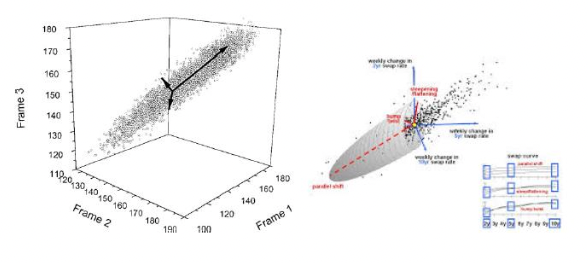
\includegraphics[width=1\textwidth,height=\textheight]{figs/Aula07/3D.png}

}

\end{figure}

\hypertarget{distuxe2ncia-estatuxedstica-em-k-dimensuxf5es-1}{%
\subsection{\texorpdfstring{Distância estatística em \(k\)
dimensões}{Distância estatística em k dimensões}}\label{distuxe2ncia-estatuxedstica-em-k-dimensuxf5es-1}}

\begin{itemize}
\tightlist
\item
  \(\Sigma\) é a matriz de covariância \(k \times k\) de um vetor
  aleatório \(Y\) de dimensão \(k\), temos

  \begin{itemize}
  \tightlist
  \item
    sempre temos \(k\) autovetores \textbf{ORTOGONAIS} entre si
  \item
    autovalores são sempre \textbf{REAIS} e \textbf{POSITIVOS}
  \end{itemize}
\item
  Esta afirmação é consequência do teorema espectral
\item
  Para todo ponto \(y\) que não seja o vetor esperado \(\mu\), queremos
  que a distância \(d^2(y,\mu)\) seja \(>0\)
\item
  Uma matriz com essa propriedade é chamada de \emph{positiva definida}
\end{itemize}

\hypertarget{norma-s}{%
\subsection{Norma-S}\label{norma-s}}

Seja \(S\) uma matriz simétrica e definida positiva

\begin{tcolorbox}[enhanced jigsaw, title=\textcolor{quarto-callout-note-color}{\faInfo}\hspace{0.5em}{Definição Norma-S}, arc=.35mm, left=2mm, leftrule=.75mm, toprule=.15mm, colbacktitle=quarto-callout-note-color!10!white, bottomrule=.15mm, rightrule=.15mm, titlerule=0mm, breakable, colframe=quarto-callout-note-color-frame, opacitybacktitle=0.6, toptitle=1mm, opacityback=0, colback=white, bottomtitle=1mm, coltitle=black]
\[\Vert x\Vert_S = x^\top S x = \sum_{i,j}x_ix_jS_{ij}\]
\end{tcolorbox}

\hypertarget{norma-de-matrizes}{%
\subsection{Norma de matrizes}\label{norma-de-matrizes}}

Vamos querer comparar ``tamanhos'' de matrizes Como atribuir um tamanho
para as matrizes abaixo?

\[\begin{bmatrix}0.1 &&\\ &0.2&\\&&0.3\end{bmatrix}\,  \begin{bmatrix}150 &&\\ &150&\\&&180\end{bmatrix}\, \begin{bmatrix}100 &80&80\\ 90&150&100\\90&100&180\end{bmatrix}\]

\hypertarget{qual-o-tamanho-quem-uxe9-maior}{%
\subsection{Qual o tamanho? Quem é
maior?}\label{qual-o-tamanho-quem-uxe9-maior}}

\[\begin{bmatrix}1 &&\\ &1&\\&&1\end{bmatrix}\,  \begin{bmatrix}1000 &\\ &1000\end{bmatrix}\, \begin{bmatrix}1.3 &5.9&-1.6\\ 1.7&6.1&9.7\\2.7&9.1&1.2\\-0.4&2.7&2.8\\2.2&7.2&7.9\end{bmatrix}\]

\hypertarget{norma-de-frobenius}{%
\subsection{Norma de Frobenius}\label{norma-de-frobenius}}

A mais simples de todas: - Empilhe as colunas da matriz como um vetor e
calcule sua norma L2

\[A = \begin{bmatrix}1.3&5.9&-1.8\\1.7&6.1&9.7\end{bmatrix}\]

\[\Vert A\Vert_F = \sqrt{(1.3)^2+(5.9)^2+(-1.8)^2+(1.7)^2+(6.1)^2+(9.7)^2}\]

\[\Vert A\Vert_F = \sqrt{\sum_{ij}\vert a_{ij}\vert^2}\]

\hypertarget{frobenius-via-linhacoluna}{%
\subsection{Frobenius via
linha/coluna}\label{frobenius-via-linhacoluna}}

Outras descrições úteis de Frobenius

\[A_{n\times m} = \begin{bmatrix}\vert&\vert&&\vert\\ a_1&a_2&\ldots&a_m\\\vert&\vert&&\vert\end{bmatrix} = \begin{bmatrix}-&b_1^\top&-\\-&b_2^\top&-\\&\vdots&\\ -&b_n^\top&-\end{bmatrix} \]

\begin{align}
\Vert A \Vert_F^2 &= \sum_{ij}\vert a_{ij}\vert^2\\
&= \sum_{j=1}^m \Vert a_j\Vert_2^2\\
&= \sum_{i=1}^n \Vert b_i^\top\Vert_2^2\\ 
&= \text{trace}(A^\top A)
\end{align}

\hypertarget{normas-de-matrizes}{%
\subsection{Normas de matrizes}\label{normas-de-matrizes}}

A norma de uma matriz é uma função \(\Vert \star\Vert\) do conjunto de
todas as matrizes complexas (de todas as ordens finitas) para
\(\mathbb R\) que satisfaz as seguintes propriedades

\begin{itemize}
\tightlist
\item
  \(\Vert A\Vert \le 0\) e \(\Vert A \Vert = 0 \Leftrightarrow A = 0\)
\item
  \(\Vert \lambda A\Vert = \vert \lambda\vert \Vert A \Vert\) para todos
  escalar \(\lambda\)
\item
  \(\Vert A + B \Vert \le \Vert A \Vert + \Vert B \Vert\) para matrizes
  do mesmo tamanho
\item
  \textbf{\(\Vert AB\Vert \le \Vert A \Vert \Vert B \Vert\) para todas
  as matriz compatíveis }
\end{itemize}

\hypertarget{normas-induzidas}{%
\subsection{Normas induzidas}\label{normas-induzidas}}

\begin{itemize}
\tightlist
\item
  Uma norma qualquer para vetores do \(\mathbb R^n\) induz uma norma no
  espaço das matrizes \(m\times n\)
\item
  Seja \(C\) conjunto dos \(x\) em \(\mathbb R^n\) tais que
  \(\Vert x \Vert = 1\)
\item
  Seja \(A\) uma matriz \(m\times n\) qualquer, então
\end{itemize}

\[ \Vert A \Vert = \max_{x\in C}{\Vert Ax\Vert}\]

\hypertarget{interpretauxe7uxe3o}{%
\subsection{Interpretação}\label{interpretauxe7uxe3o}}

\(\Vert A\Vert\) é a extensão máxima que um vetor em \(C\) pode ser
``espichado''

\begin{figure}

{\centering 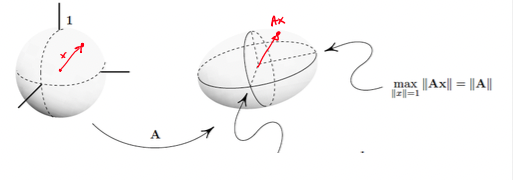
\includegraphics[width=1\textwidth,height=\textheight]{figs/Aula07/norma_interpretacao.png}

}

\end{figure}

\hypertarget{norma-espectral-induzida-pela-norma-vetorial-euclidiana}{%
\subsection{Norma espectral (induzida pela norma vetorial
euclidiana)}\label{norma-espectral-induzida-pela-norma-vetorial-euclidiana}}

\begin{itemize}
\tightlist
\item
  A norma matricial induzida pela norma vetorial euclidiana é
\end{itemize}

\[ \Vert A \Vert^2 = \max_{\Vert x\Vert^2 = 1}{\Vert Ax\Vert^2 = \sqrt{\lambda_{\text{max}}}}\]

onde \(\lambda_{\text{max}}\) é o maior autovalor tal que
\(A^\top A-\lambda I\) é singular



\end{document}
